%! subsection은 세미나를 위해 작성한 것으로, 없애거나 다른 제목으로 지울 예정.

%? 서론 스토리 진행이 자연스러운가?

\chapter{서론}

% - 많은 기업 내 직원들이 화상회의 서비스를 사용하고 있다. [1, 2]
% - 이들은 화상회의 영상 유출 사고로 피해를 받을 수 있다. [3, 4]
% - 화상회의용 워터마크로 피해를 줄일 수 있다. [5, 6]
% - 현재 화상회의용 워터마크에는 ~~한 것들이 있다. [7]
% - 이 워터마크들은 ~~한 한계가 있고, 이를 해결할 기술이 필요하다. [8, 9]

\section{배경}

\iffalse
    이 제품은 누구를 위한 것이고, 왜 그가 중요한가? - 기업을 위한 것. 많은 직원이 화상회의 서비스를 사용하고 있다.
    그는 어떤 문제가 있고, 이 문제가 왜 중요한가? - 화상회의 영상 유출 사고가 있다. 영상은 기업 자산이므로 피해를 받을 수 있다.
\fi
오늘날 많은 기업이 화상회의 서비스를 사용하고 있다. 기업은 코로나 엔데믹
이후에도 여전히 재택근무나 원격근무를 추진하고 있고, 화상회의 서비스를 사용하는
직원은 계속해서 증가하고 있다. 기업은 이런 상황 속에서 화상회의와 관련한 보안을
강화해야한다. 특히, 화상회의 영상 유출 사고는 기업에 큰 피해를 줄 수 있다. 

\iffalse
    이 제품은 무엇이며, 이 제품이 왜 중요한가? - 워터마크 기술이다. 워터마크 기술로 영상 유출을 예방하고 피해를 줄일 수 있다.
\fi
워터마크는 화상회의 영상 유출을 예방하고, 유출 피해를 줄일 수 있는
기술이다. 화상회의용 워터마크 기술은 일반적으로 화상회의 영상 소유권을 보호하기
위해 사용한다. 화상회의 화면에 회의를 개설한 사용자(이하 호스트) 정보를
워터마크로 삽입하면, 모든 회의 참석자가 워터마크가 포함된 화면만 볼 수 있다.
회의 참석자 중 누군가 화면을 녹화하고 영상을 유출하면, 유출 영상으로부터
워터마크를 추출하여 이 영상이 호스트의 것임을 보일 수 있다. 

\iffalse
    이 제품은 어떤 것이 있는가? - Zoom이 제공하는 워터마크 기술.
\fi
대표적인 화상회의 서비스 Zoom는 워터마크 기술을 사용자에게 제공하고 있다. Zoom
워터마크 기술은 호스트 이메일을 모든 회의 참석자 화면에 띄워 참석자가 이메일을 볼 수
있다. 그림 \ref{fig:zoom_wm}은 Zoom에서 워터마크 기능을 사용했을 때 보이는
화상회의 화면이다.
\begin{figure}[ht]
    \vspace{10pt}
    \centering
    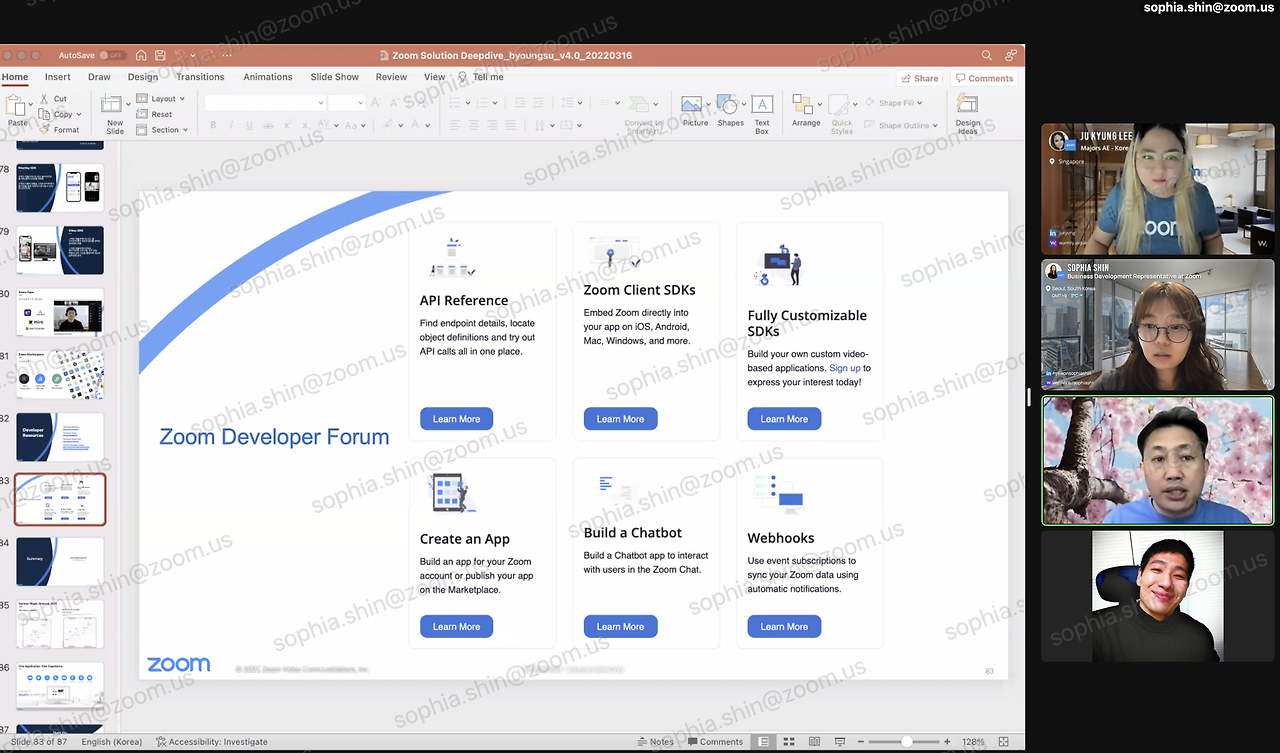
\includegraphics[width=0.7\textwidth]{imgs/zoom_wm.png}
    \caption{Zoom에서 워터마크를 삽입한 화상회의 화면}
    \label{fig:zoom_wm}
\end{figure}
Zoom 외에도 워터마크 기술을 제공하는 화상회의 서비스가 존재하며, 대부분 호스트의
식별정보를 워터마크로 사용한다. 이 워터마크 기술은 누군가 회의영상을
유출하더라도, 워터마크를 추출하여 영상 소유권이 호스트에 있음을 알 수 있다.
화상회의 서비스가 제공하는 워터마크 기술 외에도 많은 화상회의용 워터마크 기술이
존재한다. 이는 부록 \ref{apdx:aa}를 참고한다.

\section{목적}

\iffalse
    카멜레온 목적:
        1. 워터마크로부터 영상의 출처를 알 수 있도록 하기.
        2. 워터마크 메시지를 신뢰할 수 있도록 하기.
        3. 워터마크가 지워지지 않도록 하기.
    왜 이런 목적을 달성해야 하는지 설명해야한다. 기존 제품의 한계점을 언급할 수 있다.
\fi

기존 워터마크 기술에는 세 가지 한계점이 있다.

\begin{itemize}
    \item \textbf{출처 확인 불가능.} 기존 화상회의용 워터마크 기술은 회의 호스트
    식별 정보만 메시지로 사용한다. 호스트를 제외한 회의 참석자가 회의 화면을
    녹화하면, 녹화 영상에는 호스트 식별 정보만 워터마크로 삽입된다. 이 영상이
    유출되면, 유출 영상으로부터 호스트가 누구인지 알 수 있지만, 영상이
    어디로부터 유출됐는지, 누가 녹화한 영상인지 알 수 없다. 이 경우 유출 사고에
    대해 누구도 책임을 물을 수 없다. 또한 유출 출처를 막을 수 없어, 같은
    출처에서 또 다른 영상이 유출될 수 있다.
    \item \textbf{메시지 진위성 확인 불가능.} 워터마크는 신뢰할 수 있는 정보여야
    한다. 만약 워터마크에 들어가 있는 호스트 식별정보가 다른 사람의 식별정보로
    대체될 수 있다면, 유출 영상이 호스트의 것임을 확신할 수 없다. 기존
    워터마크는 메시지 진위성을 확인하는 과정이 없으므로, 워터마크를 신뢰할 수
    없다.
    \item \textbf{워터마크 삭제 가능.} 원본 영상을 손상하지 않고 워터마크를
    훼손하면, 워터마크 기능은 효력을 잃는다. 따라서 기존 워터마크는 쉽게 지울 수
    없도록 반투명화하여 콘텐츠에 삽입한다. 그러나 AI를 기반으로 한 워터마크 제거
    도구는 전문지식 없이도 기존 워터마크를 쉽게 지울 수 있다.[] 그림
    \ref{fig:wm_removed}는 AI 제거 도구를 사용하여 워터마크를 지운 화상회의
    사진이다.
    \begin{figure}[ht]
        \vspace{10pt}
        \centering
        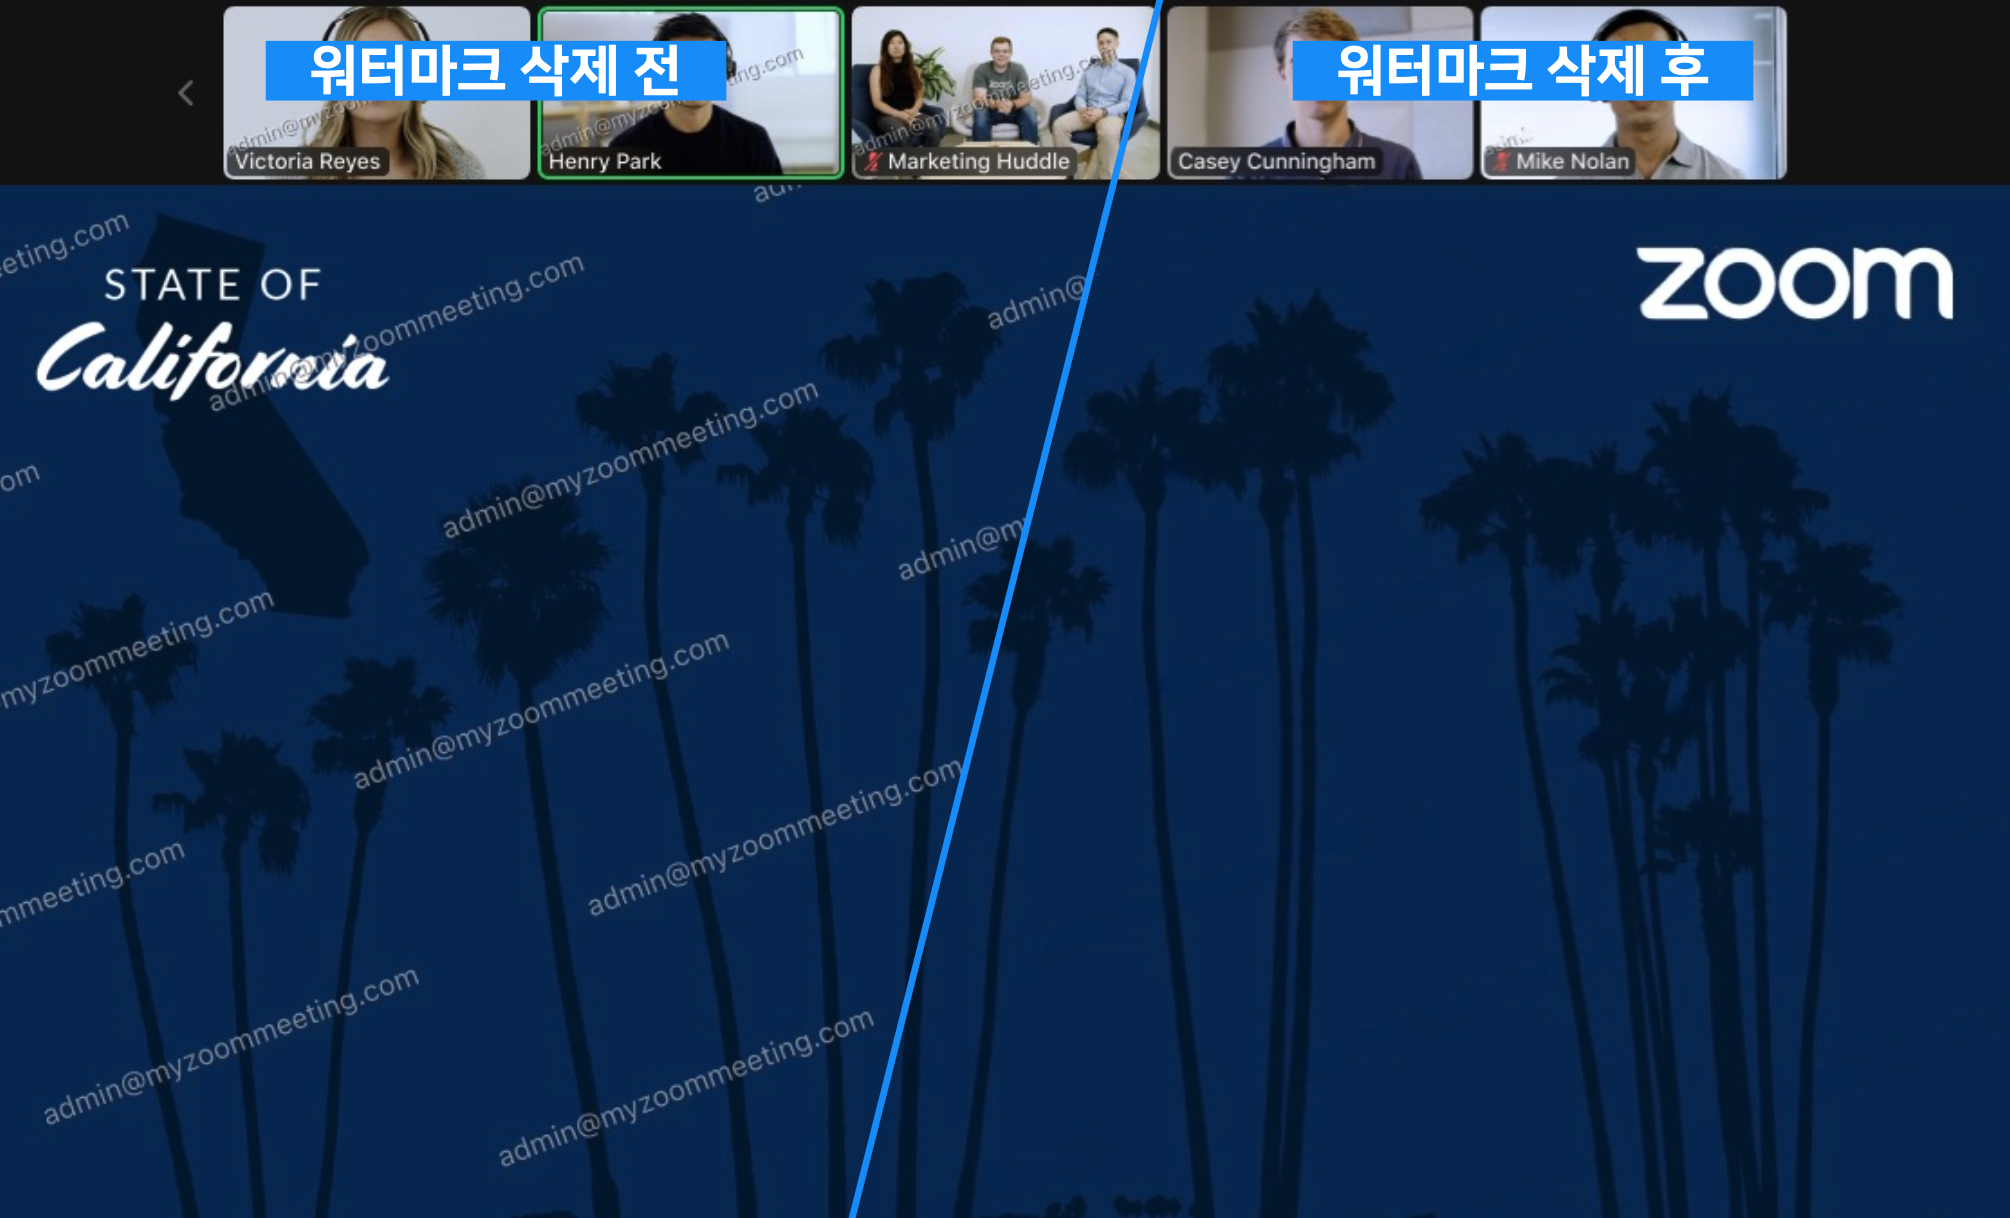
\includegraphics[width=0.7\textwidth]{imgs/wm_removed.png}
        \caption{AI 제거 도구로 Zoom 워터마크를 제거한 화상회의 화면}
        \label{fig:wm_removed}
    \end{figure}
\end{itemize}

화상회의 서비스 사용자가 기존 워터마크 기술을 사용하더라도 세 한계점 때문에
회의영상을 강하게 보호할 수 없다. 따라서 이를 해결하기 위한 개선된 워터마크
기술이 필요하다. 본 보고서에서 설명하는 워터마크 기술(이하 카멜레온)은 한계점을
극복한 개선된 워터마크 기술이다. 카멜레온은 출처와 진위성을 확인할 수 있고 AI
공격에도 견고하여, 기업은 화상회의 서비스를 보다 안전하게 사용할 수 있다.

\section{범위}

\iffalse
    카멜레온 범위:
        0. 이건 가능하다.
        1. 카멜레온은 카메라를 고려하지 않았다.
        2. 오디오 워터마크를 사용하지 않았다. 그러나 이는 독립적으로 개발 가능하다.
\fi
카멜레온은 호스트 정보뿐 아니라 회의 참석자 정보도 메시지로 사용한다. 유출한
회의영상이 가지는 워터마크로부터 참석자 정보를 확인하여 영상 출처를 알 수 있다.
카멜레온은 메시지의 진위성을 확인할 수 있는 정보를 생성하고, 워터마크로
삽입한다. 이 정보는 유출 영상에서 추출한 워터마크를 신뢰할 수 있는 증거라고 할
수 있다.

카멜레온은 AI 공격에 대응하기 위해 문자 형태 워터마크와 그림 형태 워터마크 두
가지를 사용한다. 문자 워터마크는 기존에 존재하는 워터마크 기술과 비슷하며, 그림
워터마크는 QR 코드를 활용한다. 두 종류 워터마크를 사용하면 AI는 두 워터마크를
전부 지우지 못하거나, 지우더라도 원본을 크게 훼손하여 영상 가치가 사라진다.
QR 코드 워터마크는 AI 공격 내성을 가질 수 있지만, PC 녹화기능이 아닌 외부에서
카메라로 녹화할 경우 추출이 어렵다.